
\documentclass[ms.tex]{subfiles}
\begin{document}

\section{Application to the H3 Survey}
\label{sec:h3}

\begin{itemize}

	\item Next we apply our fitting method to two dwarf satellite remnants
	observed in the Milky Way halo: the Gaia-Sausage Enceladus (GSE) and the
	Sagittarius (Sgr) dwarf Spheroidal (dSph).
	We choose these systems because they probe two qualitatively different SFHs.
	The GSE exhibits smooth, monotonic trends of~\afe~with~\feh~(see
	Fig.~\ref{fig:gse_bestfit} and discussion in~\S~\ref{sec:h3:gse} below),
	an empirical result which does not demand a sudden event such as a
	starburst in its explanation.
	The Sgr dSph, on the other hand, exhibits an increase in~\afe~which is
	accompanied by an increase in the observed density of stars (see
	Fig. X and discussion in~\S~\ref{sec:h3:sgr} below).
	This result, contrary to the GSE data, is naturally explained by a burst in
	star formation.

\end{itemize}

\subsection{The H3 Survey}
\label{sec:h3:survey}

\subsection{The Gaia-Sausage Enceladus}
\label{sec:h3:gse}

\begin{figure*}
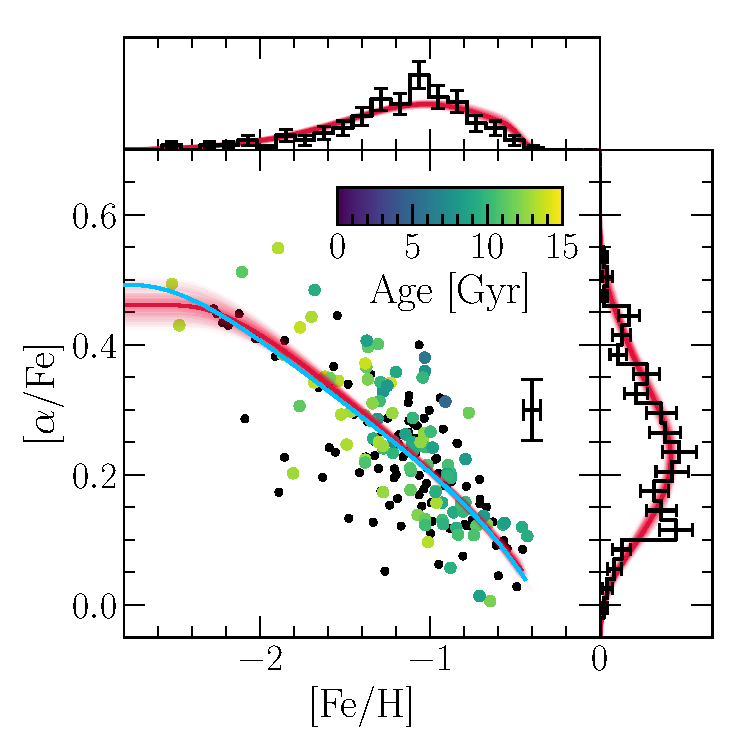
\includegraphics[scale = 0.5]{gsefit_afe_feh.pdf}
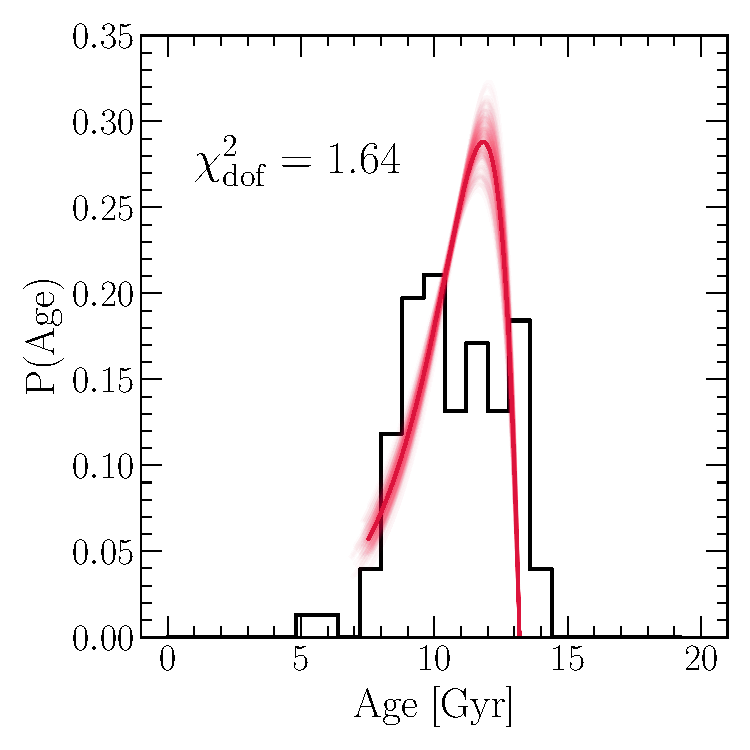
\includegraphics[scale = 0.42]{gsefit_agedist.pdf}
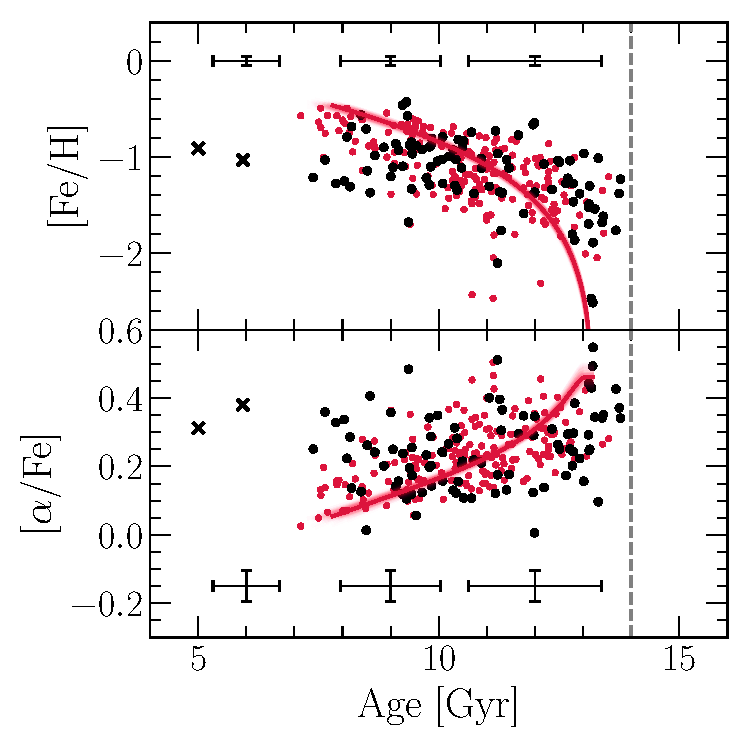
\includegraphics[scale = 0.42]{gsefit_amr.pdf}
\caption{
\textbf{Left}: The~\afe-\feh~plane and associated marginalized distributions.
Stars are colour-coded according to their age where available and are otherwise
plotted in black.
The best-fit chemical evolution track and distributions in~\afe~and~\feh~are
shown as solid red lines.
The median~\feh~and~\afe~errors of the sample are shown by the error bar to the
right of the data. 
\textbf{Middle}: The age distribution measured for our GSE sample (black) and
the best-fit age distribution based on the SFH of our model (red, solid).
We additionally plot the age distribution obtained when we convolve the best-fit
distribution with an uncertainty of~$\sigma(\log_{10}(\text{age}))$ including
the prior that age~$<$ 14 Gyr as in the H3 age measurements.
\textbf{Right}: The age-\feh~and age-\afe~relations of our GSE sample (black)
and our best-fit chemical evolution model (red).
The median~\feh,~\afe, and age uncertainties are shown by the error bars to the
left of the data in each panel.
We plot the two stars that we exclude from our fit as our black X's (see
discussion in~\S~\ref{sec:h3:gse}).
In all panels, we subsample 200 sets of parameter choices~$\{\theta\}$ from our
likelihood distribution (see Fig.~\ref{fig:gse_corner}) and plot their
predictions as high transparency lines to provide a sense of the fit precision
in the observed space.
}
\label{fig:gse_bestfit}
\end{figure*}

\begin{figure*}
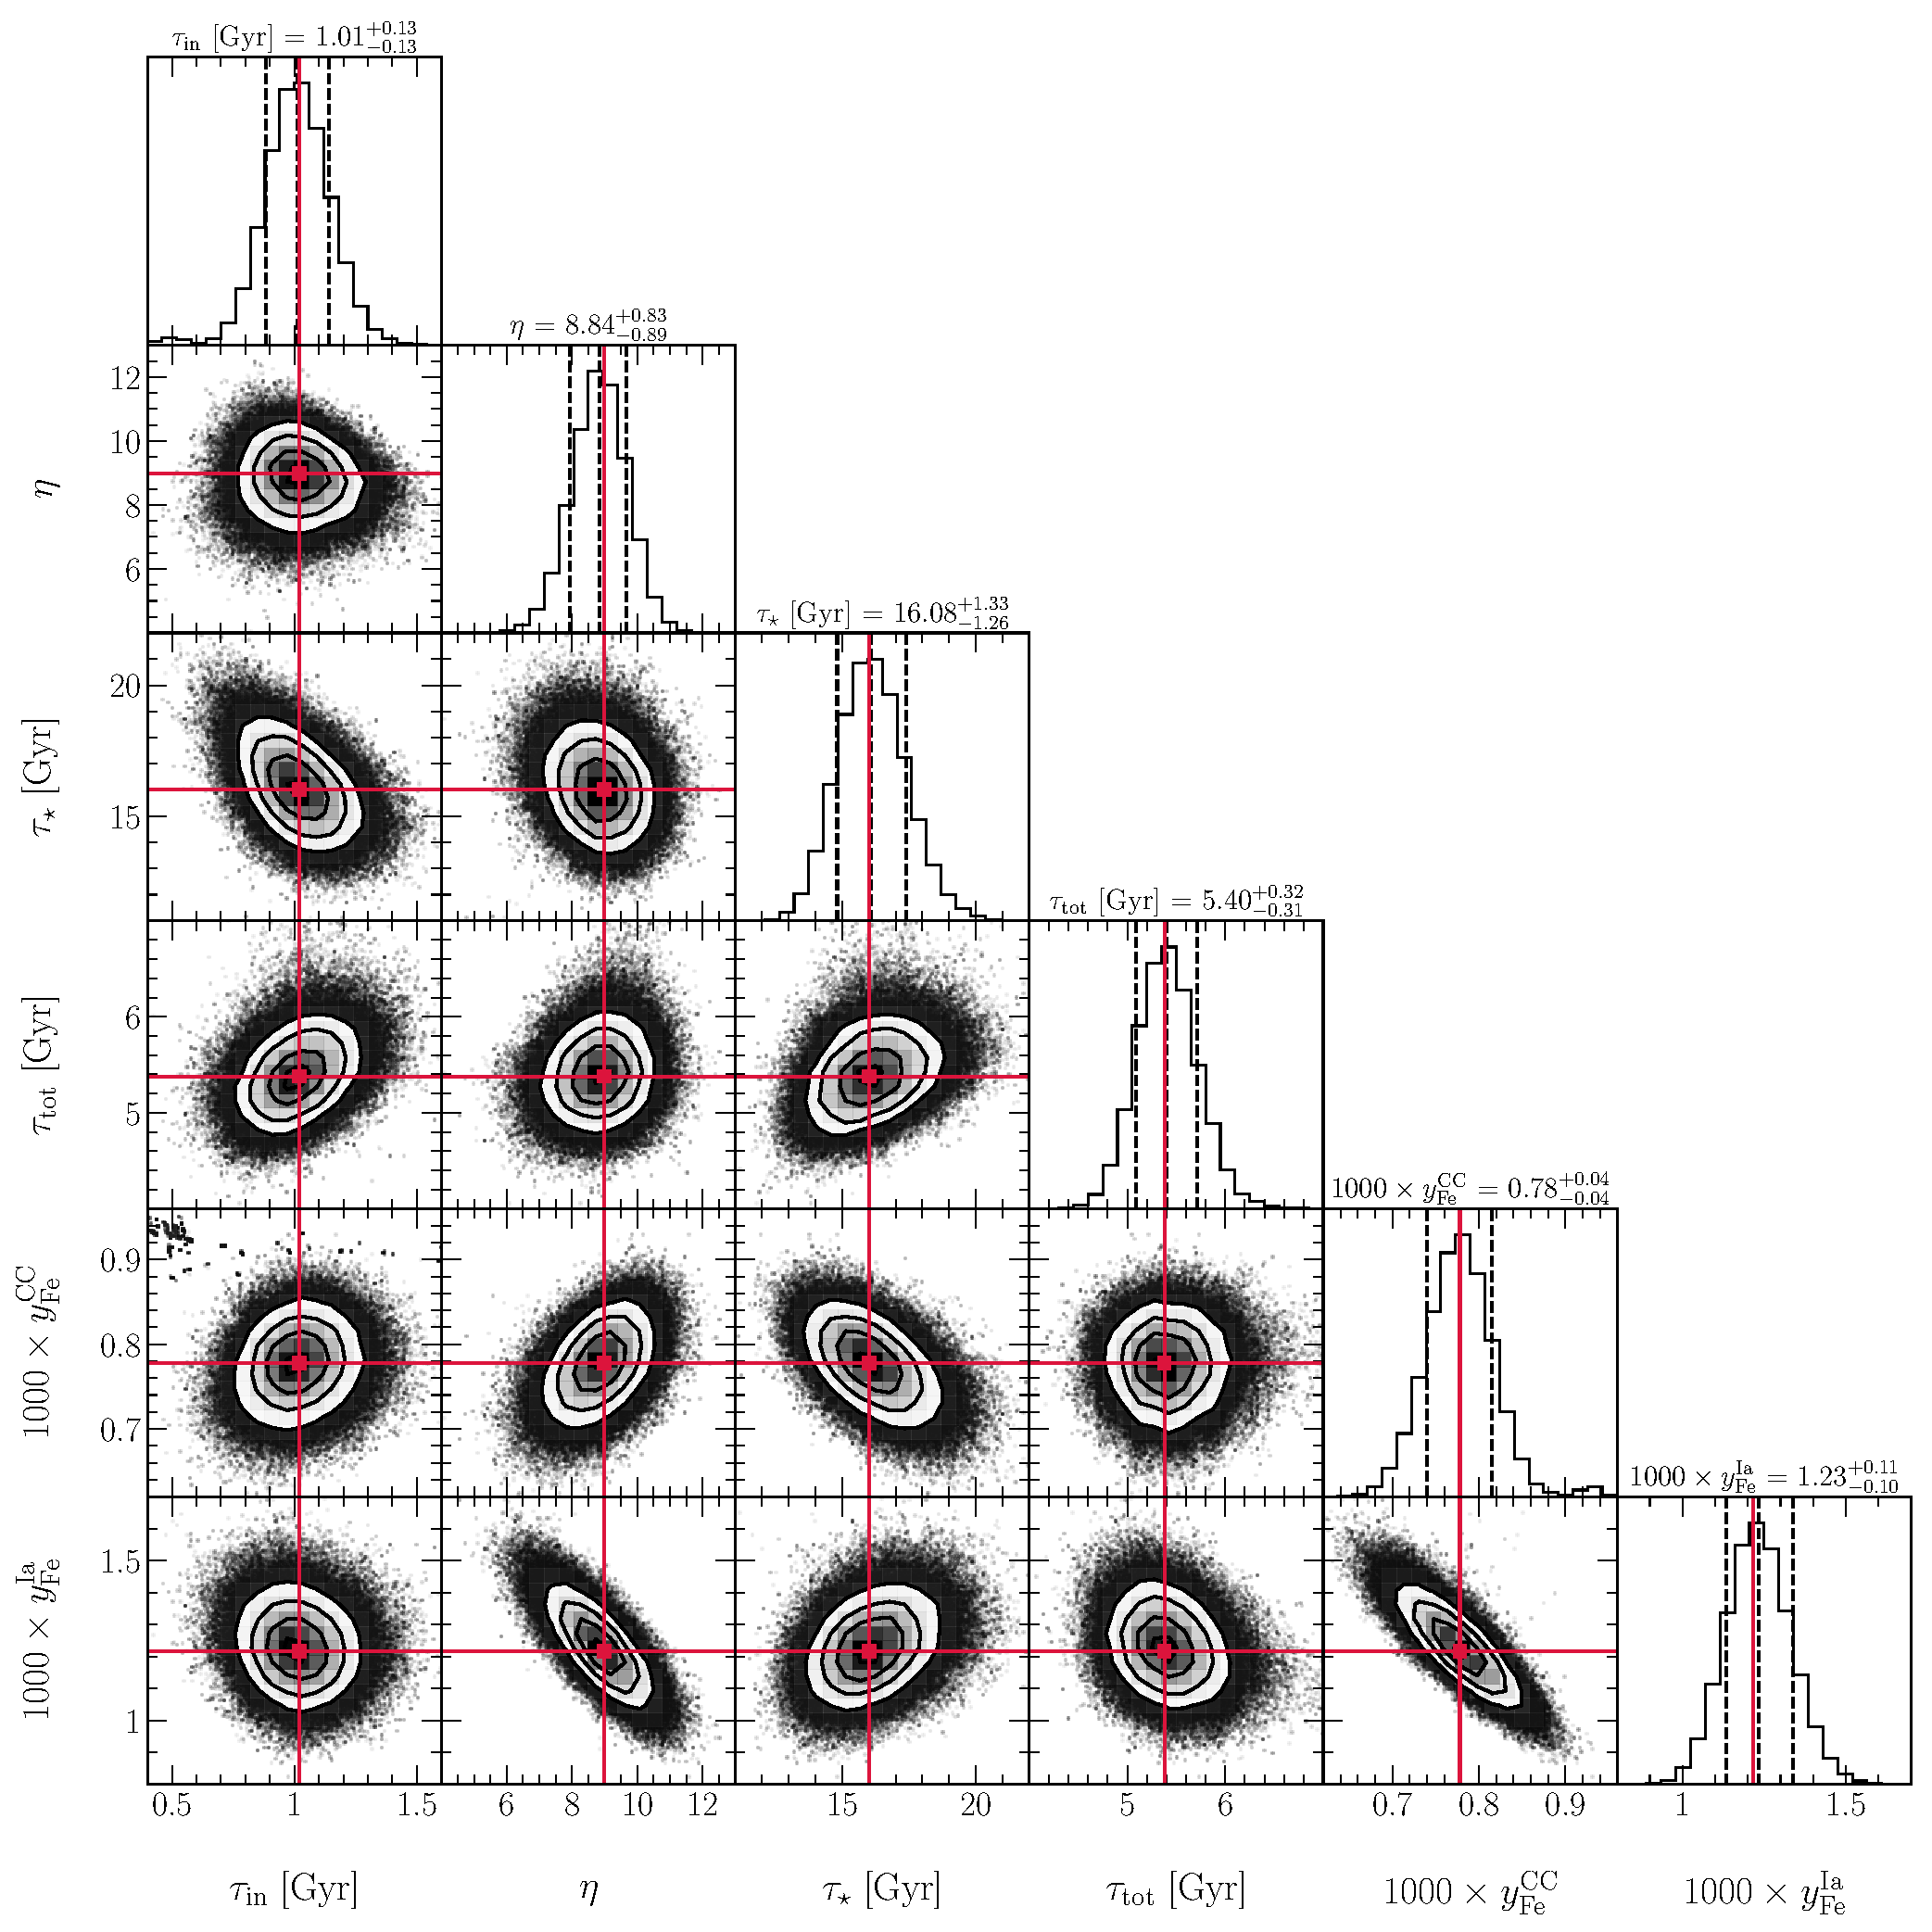
\includegraphics[scale = 0.45]{gsechem_512k.pdf}
\caption{
The ``corner-plot'' showing the results of our fitting method applied to GSE
stars observed by the H3 survey.
We show the marginalized likelihood distributions in each parameter along with
their best-fit values and confidence intervals along the diagonal.
Below the diagonal, we show the 2-dimensional cross-sections of the
6-dimensional likelihood function.
Contrary to Fig.~\ref{fig:corner_fiducial}, red ``cross-hairs'' mark the
element of the Markov chain with the maximum statistical likelihood.
}
\label{fig:gse_corner}
\end{figure*}

\begin{itemize}

	\item Our sample from the GSE consists of 189 stars, 95 of which have
	age measurements.
	These stars span metallicities of~$\feh \approx -2.5$ to~$-0.4$ and
	$\afe \approx 0$ to $+0.55$.
	Abundance uncertainties range from~$\sim$0.02 to~$\sim$0.12 in
	both~\feh~and~\afe~with median values near~$\sim$0.05.
	Of the stars with age measurements, the youngest is~$\sim$5 Gyr old and the
	oldest is~$\sim$13.8 Gyr old.
	All inferred ages, however, incorporate a prior imposed by the H3 pipeline
	which requires all values to be below 14 Gyr, preventing the log-normal
	nature of age uncertainties from populating the~$\sim14 - 20$ Gyr range.
	Every age measurement has a statistical uncertainty below
	$\sigma(\log_{10}(\text{age})) = 0.05$, corresponding to a measurement
	precision of~$\lesssim$12\%.
	Due to the difficulty associated with measuring stellar ages both
	accurately and precisely (refs), we adopt this value of
	$\sigma(\log_{10}(\text{age})) = 0.05$ as the minimum uncertainty to
	account for any systematic errors that may be present.
	This consequently applies to the whole subset of our sample that has age
	measurements.

	\item The left panel of Fig.~\ref{fig:gse_bestfit} shows our sample in
	the~\afe-\feh~plane along with the associated marginalized distributions.
	The mode of the MDF is near~$\feh = -1$ and~$\afe = +0.25$, and the
	``knee'' associated with the onset of SNe ia enrichment is apparent
	near~$\feh \approx -2$, though there are only a few stars in our sample
	in this region of chemical space.
	Invoking the equilibrium arguments of~\citet{Weinberg2017}, the knee
	occurring at low metallicity and an MDF dominated by low metallicity stars
	is indicative, respectively, of slow star formation (i.e. high~$\tau_\star$)
	and a low equilibrium abundance due to strong outflows (i.e. high~$\eta$).
	This is expected for a dwarf galaxy progenitor where star formation is
	typically slow~\citep[e.g.][]{Hudson2015} and the gravitational potential
	well is shallow due to low stellar and halo masses.
	Furthermore, the alpha-enhanced nature of the MDF is indicative of an SFH
	which was truncated early in the GSE's history before SN Ia enrichment
	could produce enough Fe to reach solar~\afe, a result which also expected
	given that the GSE is known to host old stellar populations (refs).

	\item In the middle and right panels, we show the age distribution,
	age-\feh~relation, and age-\afe~relation.
	The age distribution is dominated by old stars ($\gtrsim$8 Gyr), consistent
	with previous studies of the GSE (refs).
	The truncation of the age distribution likely reflects the quenching of
	star formation in the GSE progenitor by ram pressure stripping at the time
	of its first infall into the Milky Way (refs).
	The age-metallicity relation (AMR), both age-\feh~and age-\afe, has a
	considerable amount of scatter, in large part because of the considerable
	age uncertainties compared to the abundance uncertainties.

	\item We note the presence of two outliers at ages of~$\sim$5 and 6 Gyr,
	marked by X's in the right panel.
	These stars have abundances typical of the rest of the GSE population but
	are anomalously young.
	It's likely that these are blue stragglers: stars which are thought to be
	made hotter and more luminous by accretion from a binary companion.
	As a result, they occupy a region of the CMD which is normally occupied by
	much younger, more massive stars, biasing their age measurements to low
	values~\citep[e.g.][]{Bond1971, Stryker1993}.
	We therefore omit these stars from our chemical evolution model fit to the
	GSE, including only those which are older than~$\sim$7 Gyr.

	\item The steadily sloped decline of~\afe~with increasing~\feh~and the
	approximately monotonic nature of the age-\feh~and age-\afe~relations
	incidicate a smooth SFH.
	If the GSE had experienced a burst in star formation at some point in its
	history, this would be accompanied by a sudden increase in~\afe~followed by
	a decline back toward the pre-burst value due to the temporarily perturbed
	ratio of CCSN and SN Ia rates~\citep{Johnson2020}.
	We therefore fit the GSE with a smooth evolutionary model, adopting the
	same exponential infall history as our mock samples described
	in~\S~\ref{sec:mocks:fiducial}.

	\item Fig.~\ref{fig:gse_corner} shows the likelihood distribution we obtain
	for the GSE by applying our fitting method.
	We indeed find that the best-fit evolutionary model implies slow star
	formation ($\tau_\star \approx 16$ Gyr) and strong outflows
	($\eta \approx 9$), qualitatively similar to our mock samples.
	Our fit additionally suggests that the Fe yields are
	$\yfecc = \scinote{7.78^{+0.37}_{-0.38}}{-4}$ and
	$\yfeia = \scinote{1.23^{+0.11}_{-0.10}}{-3}$ on the scale where the alpha
	element yield is fixed at~$\yacc = 0.01$.
	With these Fe yields, our fit to the GSE data suggests that CCSNe account
	for~$\yfecc / (\yfecc + \yfeia) \approx$ 40\% of the Fe in the universe.
	As discussed in~\S~\ref{sec:onezone:yields} and quantified in Appendix
	\ref{sec:yield_outflow_degeneracy}, these yields are subject to the
	yield-outflow degeneracy along with~$\eta$ and~$\tau_\star$, and our
	adopted value of~$\yacc = 0.01$ is only intended to set some overall scale
	to these values which can be adjusted as necessary.
	Consequently, only relative rather than absolute values carry any meaning.
	In the absence of winds (i.e.~$\eta = 0$) but with otherwise the same
	evolutionary parameters, the MDF is predicted to have a peak
	near~$\feh \approx -0.5$ with a tail toward low metallicities and a
	sharp cutoff at higher metallicities, indicating that star formation in the
	GSE was slow enough that it would have only achieved~$\sim$one-third solar
	metallicity within 5.4 Gyr of star formation even with the largest sink
	term in the enrichment rates removed.
	If star formation instead sped up to~$\tau_\star = 1$ Gyr, corresponding
	approximately to the expected value if the GSE were composed entirely of
	molecular hydrogen while forming stars at~$z \gtrsim 1$~\citep{Tacconi2018},
	then the MDF is still peaked near~$\feh \approx -1$ but is more symmetric
	and less skewed toward lower~\feh~as in the GSE data (see
	Fig.~\ref{fig:gse_bestfit}).
	In order to predict an MDF dominated by solar metallicity stars, this model
	requires~\textit{both} weaker outflows and more efficient star formation.

	\item The infall timescale~$\tau_\text{in}$ and the total duration of
	star formation~$\tau_\text{tot}$, however, are orthogonal to the
	yield-outflow degeneracy (see Appendix~\ref{sec:yield_outflow_degeneracy}),
	indicating that these absolute values do carry meaning.
	The infall history is sharp ($\tau_\text{in} \approx 1$ Gyr), as expected
	given the alpha-enhanced mode of the MDF.
	Star formation lasted~$5.40^{+0.32}_{-0.31}$ Gyr after an onset assumed to
	occur at a lookback time of 13.2 Gyr based on the~\textsc{UniverseMachine}
	semi-analytic model~\citep[][see discussion
	in~\S~\ref{sec:mocks:fiducial}]{Behroozi2019}.
	This corresponds to the GSE's last episode of star formation occurring
	$7.80^{+0.31}_{-0.32}$ Gyr ago, consistent with direct age constraints on
	the GSE (refs).

	\item We plot the predictions of our best-fit model over the GSE data in
	Fig.~\ref{fig:gse_bestfit}, along with 200 additional parameter choices
	selected from the Markov chain plotted as high transparency lines to
	provide a visual sense of the fit uncertainty.
	Overall, this is a reasonable fit to the
	2-dimensional~\afe-\feh~distribution as well as the age-\feh~and the
	age-\afe~relations.
	We quantify the quality of the fit in the same manner described in the
	final paragraph of~\S~\ref{sec:mocks:fiducial_fit}, finding
	$\chi_\text{dof}^2 = 1.34$.
	This suggests that although the fit describes the data reasonably well,
	there is some slight room for improvement, perhaps in the age distribution
	which our best-fit model predicts to be slightly more peaked than the data.
	To again demonstrate the intrinsic age distribution is more peaked than the
	observed age distribution due to the log-normal nature of age uncertainties,
	we sample our best-fit age distribution with~$10^4$ stars and perturb them
	with an uncertainty of~$\sigma(\log_{10}(\text{age})) = 0.05$, our adopted
	age uncertainty to account for systematics (see discussion above).
	We maintain the same prior as the H3 pipeline requireing all age sto be
	below 14 Gyr and plot the result in the middle panel of
	Fig.~\ref{fig:gse_bestfit}.
	Although age uncertainties can account for some of the differences between
	the intrinsic and observed age distributions, it is still somewhat more
	peaked.
	This suggests that the SFH of the GSE may differ from what would be implied
	by an exponential infall history, though only slightly as the fit does
	reasonably well anyway.

\end{itemize}

\subsection{The Sagittarius Dwarf Spheroidal}
\label{sec:h3:sgr}

\end{document}

